\documentclass{article}

% Language setting
% Replace `english' with e.g. `spanish' to change the document language
\usepackage[english]{babel}

% Set page size and margins
% Replace `letterpaper' with `a4paper' for UK/EU standard size
\usepackage[letterpaper,top=2cm,bottom=2cm,left=3cm,right=3cm,marginparwidth=1.75cm]{geometry}
\usepackage{bm}

% Useful packages
\usepackage{amsmath}
\usepackage{amssymb}

\usepackage{algorithm}
\usepackage{algpseudocode}
\usepackage{appendix}

\usepackage{graphicx}
\usepackage[colorlinks=true, allcolors=blue]{hyperref}

\usepackage{subcaption}

\usepackage{tikz}

% Costume Style Begin
\usepackage{enumitem}

\usepackage{listings}
\usepackage{xcolor}

\lstset{
    language=Python,
    basicstyle=\ttfamily\small,
    keywordstyle=\color{blue},
    commentstyle=\color{green!60!black},
    stringstyle=\color{red},
    tabsize=4,
    showspaces=false,
    showstringspaces=false,
    frame=single,
}
% Costume Style End

% Operator Declaration Begin

% Operator Declaration End

\title{SUSTech CS324 2024 Spring Assignment 3 Report}
\author{12110304 Chunhui XU}

\begin{document}
\maketitle

\section{Part 1 Task 1}

\subsection{Simple Introduction}

In Assignment 3, we train our model on the same data set, that is, the prediction of the palindrome structure mentioned in Assignment 2.

Of course, in Assignment 2, we tried to use RNN to solve this problem, but the results were not satisfactory: the model still performed better for shorter palindrome strings, but the performance for longer strings was somewhat different. Decline, even training results are getting worse. Therefore, in this exercise we try to use LSTM (Long Short-Term Memory) \cite{HochSchm97} with better memory ability to solve this problem.

\subsection{LSTM Structure}

\subsubsection{LSTM Formulas}

I build the LTSM with the following formulas:

\begin{align}
    g^{(t)} &= \tanh(W_{gx}x^{(t)} + W_{gh}h^{(t-1)} + b_{g})\\
    i^{(t)} &= \sigma(W_{ix}x^{(t)} + W_{ih}h^{(t-1)} + b_{i})\\
    f^{(t)} &= \sigma(W_{fx}x^{(t)} + W_{fh}h^{(t-1)} + b_{f})\\
    o^{(t)} &= \sigma(W_{ox}x^{(t)} + W_{oh}h^{(t-1)} + b_{o})\\
    c^{(t)} &= g^{(t)} \odot i^{(t)} + c^{(t-1)} \odot f^{(t)}\\
    h^{(t)} &= \tanh(c^{(t)} \odot o^{(t)})\\
    p^{(t)} &= (W_{ph}h^{(t)} + b_{p})\\
    \Tilde{y}^{(t)} &= \text{softmax}(p^{(t)})
\end{align}

where $\odot$ denotes the element-wise multiplication.

The structure is similar to that of the RNN implemented in Assignment 2, but with the addition of three gates: the input gate $i$, the forget gate $f$, and the output gate $o$ (and the input modulation $g$). I shall initialise $h^{(0)}$ to the vector of all zeros.

Use the cross-entropy loss over the last time-step:

\begin{equation}
    \mathcal{L} = -\sum\limits_{k=1}^{K}y_{k}log(\Tilde{y}_{k}^{(T)})
\end{equation}

where $k$ runs over the classes ($K = 10$ digits in total), $y_k$ is a one-hot encoding vector.

\subsubsection{\texttt{PyTorch} Implementation}

When I implement the structure, for each one among $g$, $i$, $f$, $o$, I use \texttt{nn.Linear} with bias to compute the $x^{(t)}$ part, \texttt{nn.Linear} without bias to compute the $h^{(t-1)}$ part.

In each \texttt{for} loop, for $h$ and $c$, update them with \texttt{torch} notation $*$ and \texttt{torch.tanh}.

Finally, use \texttt{nn.Linear} with bias to compute the $p^{(t)}$, and use \texttt{torch.softmax} to get the output.

\section{Part 1 Task 2}

\subsection{Simple Introduction}

In this part, I will train my LSTM on palindrome dataset with default parameters, and compare the different result with changing the \texttt{input\_length}.

\subsection{Default Parameters}

\begin{itemize}
    \item \texttt{input\_length}: $4$, length of input sequence
    \item \texttt{input\_dim}: $1$, dimension of input data
    \item \texttt{num\_classes}: $10$, number of classes in the classification task
    \item \texttt{num\_hidden}: $128$, number of hidden units in the neural network
    \item \texttt{batch\_size}: $128$, batch size for training
    \item \texttt{learning\_rate}: $0.001$, learning rate for optimization
    \item \texttt{max\_epoch}: $100$, maximum number of epochs to train the model
    \item \texttt{max\_norm}: $10$, maximum norm constraint for gradient clipping
    \item \texttt{data\_size}: $100000$, size of the dataset
    \item \texttt{portion\_train}: $0.8$, portion of the dataset used for training
\end{itemize}

I will tested the training efficiency under different $T$ values (i.e. \texttt{input\_length} + 1).

\subsection{Result Visualization}

Table \ref{tab:p1_res_para} shows different parameters and corresponding figure.

\begin{table}[!h]
\centering\caption{Different Parameters and Result}
\label{tab:p1_res_para}
\begin{tabular}{|c|c|c|}
\hline
\textbf{Fig ID} & $T$ & \textbf{Changed Parameters} \\
\hline
Fig \ref{fig:p1_t5_default} & 5 & Default Parameters \\ \hline
Fig \ref{fig:p1_t20_default} & 20 & Default Parameters \\ \hline
Fig \ref{fig:p1_t5_lr_change} & 5 & Change leaning rate to $1\mathrm{e}^{-2}$ and $1\mathrm{e}^{-4}$ \\ \hline
Fig \ref{fig:p1_t20_lr_change} & 20 & Change leaning rate to $1\mathrm{e}^{-2}$ and $1\mathrm{e}^{-4}$ \\ \hline
Fig \ref{fig:p1_t30} & 30 & Change leaning rate to $1\mathrm{e}^{-4}$ \\ \hline
Fig \ref{fig:p1_t20_rnn} & 20 & Assignment 2 RNN Network \\ \hline
\end{tabular}
\end{table}

\begin{figure}[!htbp]
    \centering
    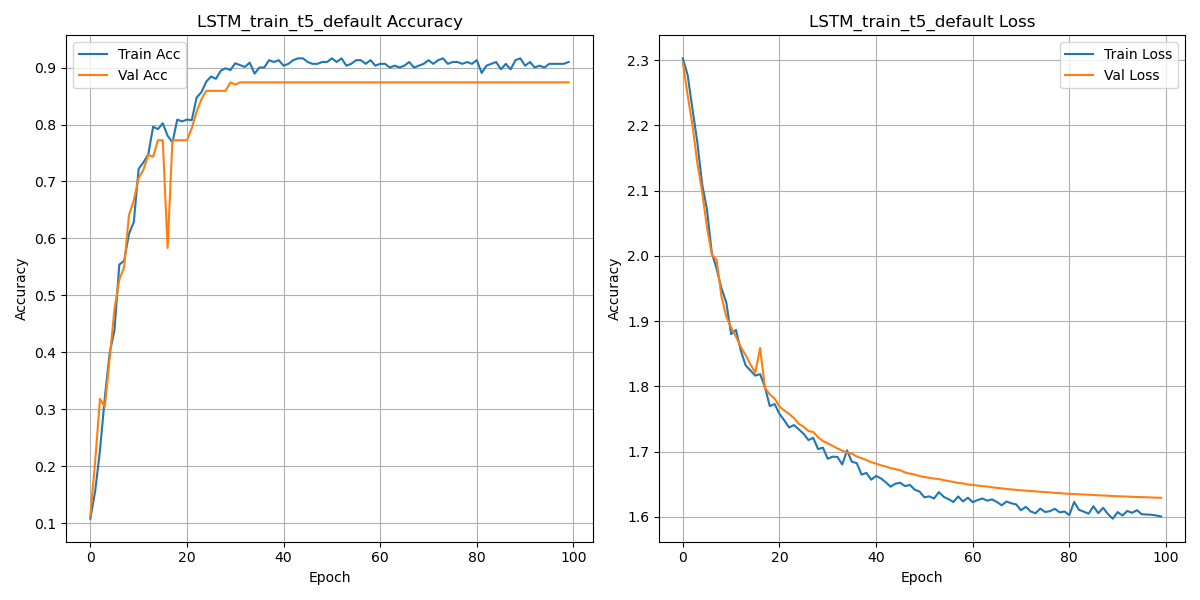
\includegraphics[width=1\textwidth]{img/part1/LSTM_train_t5_default.png}
    \caption{$T = 5$ Default Curve}
    \label{fig:p1_t5_default}
\end{figure}

\begin{figure}[!htbp]
    \centering
    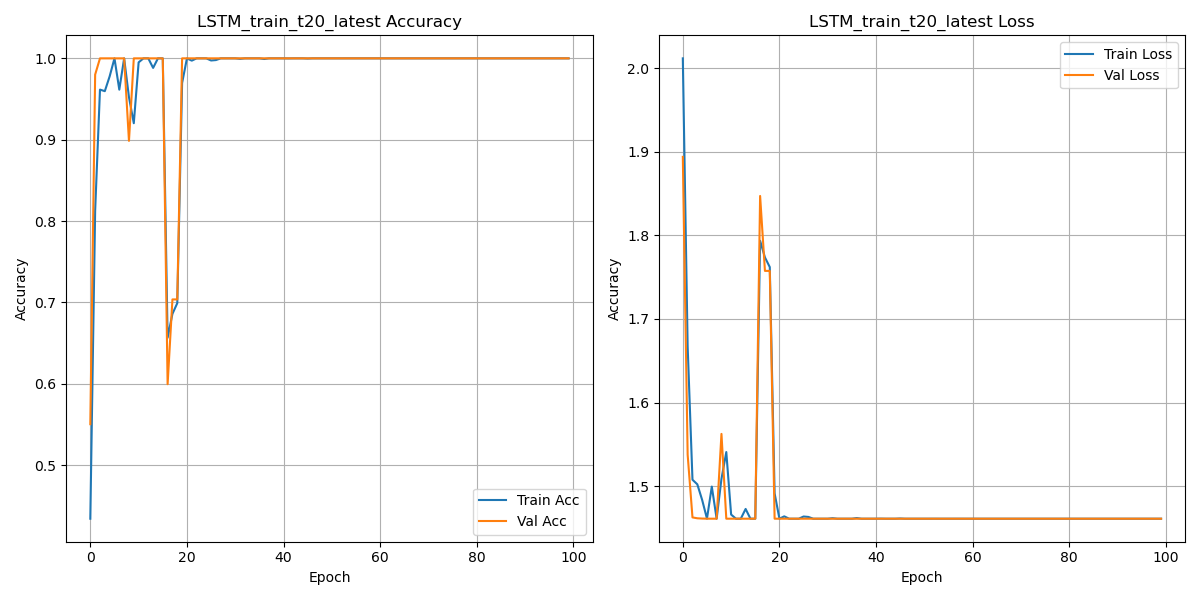
\includegraphics[width=1\textwidth]{img/part1/LSTM_train_t20_default.png}
    \caption{$T = 20$ Default Curve}
    \label{fig:p1_t20_default}
\end{figure}

\subsection{Result Analysis}

\subsubsection{Overall Analysis}

We can find that compared to RNN, LSTM not only achieves a better upper limit of accuracy on long inputs, but also has a significantly improved convergence speed. Compared with the original RNN structure, we can reasonably speculate that LSTM can achieve better training results on longer sequence inputs.

\subsubsection{Learning Rate Analysis}

By changing variables, especially the learning rate, we also found more interesting results.
\begin{itemize}
    \item For shorter inputs, a lower learning rate converges slower and has poorer learning effects; a higher learning rate can speed up the convergence and reach a higher upper limit of accuracy;
    \item For longer inputs, a lower learning rate can eventually reach a higher upper limit of accuracy; while a higher learning rate leads to model degradation, and the prediction effect fluctuates and becomes worse.
\end{itemize}

Here are the possible explanations I can think of for these situations:

\begin{itemize}
    \item Increasing the learning rate might help the model converge faster, especially early in training. For shorter inputs, a higher learning rate means faster and more efficient convergence.
    \item Reducing the learning rate can help improve the stability of the model and reduce instability during the training process. Especially when the sequence length increases, problems such as vanishing/exploding gradient are more likely to occur. By reducing the learning rate, the magnitude of parameter updates can be reduced to better deal with these problems.
\end{itemize}


\section{Part 2 Task 1}

\subsection{Simple Introduction}

In the second part of this assignment you will implement a GAN (Generative Adversarial Network) \cite{goodfellow2014generative} that generates images similar to those of the training set. The training set is MNIST handwritten digit database.

\begin{figure}[!htbp]
    \centering
    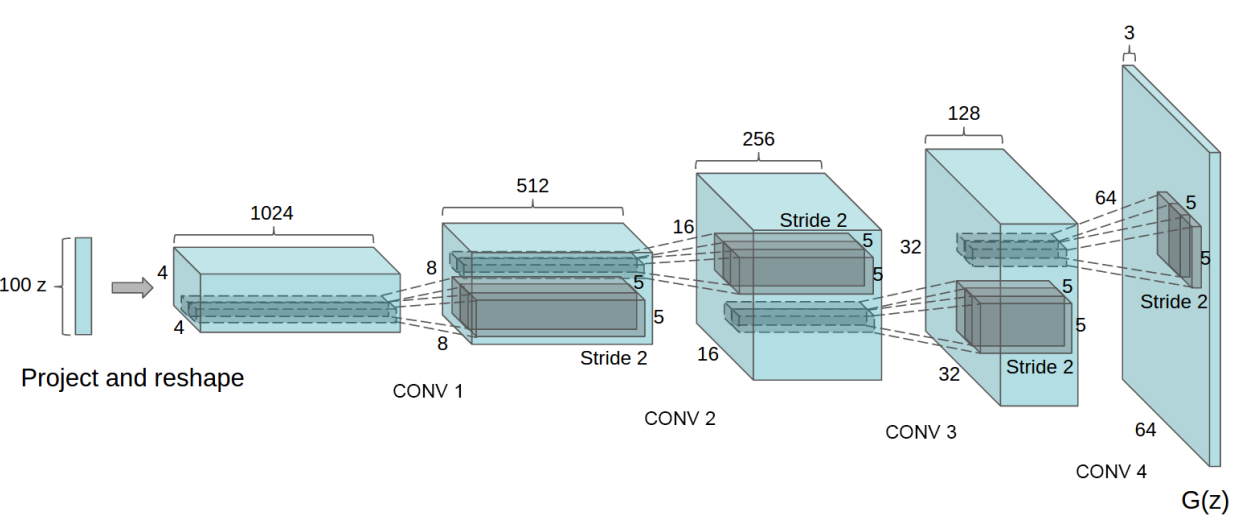
\includegraphics[width=1\textwidth]{img/p2t1/GAN_struct.png}
    \caption{A Typical GAN Structure}
    \label{fig:p2_gan_struct}
\end{figure}

\subsection{Function Analyze}

GAN is a neural network structure composed of a generator and a discriminator, designed to generate realistic data samples, such as images, text, or audio. I show the overview of the structure and training methods:

\begin{itemize}
    \item {
        Network Structure
        \begin{itemize}
            \item Generator: The generator accepts a random noise vector as input and outputs new samples similar to the training data. It usually consists of a network that turns low-dimensional noise vectors to high-dimensional data space.
            \item Discriminator: The discriminator accepts real samples and fake samples generated by the generator as input and tries to distinguish them. It usually consists of a convolutional network that is used to classify whether the input sample is a real sample or a fake sample generated by the generator.
        \end{itemize}
    }
    \item {
        Training Method

        During the training process, the generator and discriminator compete with each other and improve each other's performance through adversarial training.
        
        The training process is usually divided into two stages: first, the generator generates fake samples, and then the discriminator evaluates the authenticity of these fake samples. The feedback given by the discriminator is then used to update the parameters of the generator and discriminator.

        The goal of the generator is to generate samples that are as realistic as possible to fool the discriminator into thinking the generated samples are real. And the goal of the discriminator is to distinguish between real samples and fake samples generated by the generator as much as possible, so as to effectively detect fake samples generated by the generator.
    }
\end{itemize}

\subsection{Structure Analysis}

Training the GAN involves playing a minmax game between the generator and
discriminator. In other words, our optimization objective is

\begin{equation}
    \min\limits_{G} \max\limits_{D}V(D,G)=
    \min\limits_{G} \max\limits_{D}\mathbb{E}_{p}[\log{D(X)}] + \mathbb{E}_{q}[\log{(1-D(G(Z)))}]
\end{equation}

\subsubsection{Generator Layers}

\begin{enumerate}
    \item $100$ input, \texttt{latent\_dim}
    \item $100 \to 128 $ Linear Layer 
    \item LeakyRelu
    \item $128 \to 256 $ Linear Layer
    \item BatchNorm, LeakyReLU
    \item $256 \to 512 $ Linear Layer
    \item BatchNorm, LeakyReLU
    \item $512 \to 1024$ Linear Layer
    \item BatchNorm, LeakyReLU
    \item $1024 \to 768$ Linear Layer
    \item $768$ output, image
\end{enumerate}

\subsubsection{Discriminator Layers}

\begin{enumerate}
    \item $784$ input, a image
    \item $784 \to 512 $ Linear Layer 
    \item LeakyReLU
    \item $512 \to 256 $ Linear Layer
    \item LeakyReLU
    \item $256 \to 1 $ Linear Layer
    \item $1$ output, means real or fake
\end{enumerate}

\section{Part 2 Task 2}

\subsection{Simple Introduction}

In this part, I need sample 25 images from my trained GAN. And I will do this at the start of training, halfway through training and after training has terminated.

\subsection{Default Parameters}

\begin{itemize}
    \item \texttt{n\_epochs}: $200$, maximum number of epochs to train the model
    \item \texttt{batch\_size}: $64$, batch size for training
    \item \texttt{lr}: $0.0002$, learning rate for optimization
    \item \texttt{latent\_dim}: $100$, dimension of input noise
    \item \texttt{save\_interval}: $500$, interval for saving images generated.
\end{itemize}

I use \texttt{torch.optim.Adam()} for optimizer, \texttt{torch.nn.BCELoss()} for loss function.

\subsection{Result Visualization}

Fig \ref{fig:p2t2_train} shows the results of 25 sample images at the start of training, halfway through training and after training has terminated.

\begin{figure}[!htbp]
  \centering
  \begin{subfigure}[b]{0.3\textwidth}
    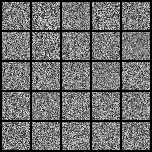
\includegraphics[width=\textwidth]{img/p2t2/0.png}
    \caption{Start ($0/187,500$)}
  \end{subfigure}
  \begin{subfigure}[b]{0.3\textwidth}
    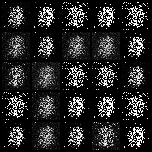
\includegraphics[width=\textwidth]{img/p2t2/1000.png}
    \caption{Start ($1,000/187,500$)}
  \end{subfigure}
  \begin{subfigure}[b]{0.3\textwidth}
    \includegraphics[width=\textwidth]{img/p2t2/10000.png}
    \caption{Start ($10,000/187,500$)}
  \end{subfigure}
  \begin{subfigure}[b]{0.3\textwidth}
    \includegraphics[width=\textwidth]{img/p2t2/20000.png}
    \caption{Middle ($20,000/187,500$)}
  \end{subfigure}
  \begin{subfigure}[b]{0.3\textwidth}
    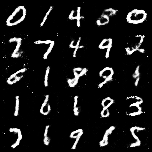
\includegraphics[width=\textwidth]{img/p2t2/90000.png}
    \caption{Middle ($90,000/187,500$)}
  \end{subfigure}
  \begin{subfigure}[b]{0.3\textwidth}
    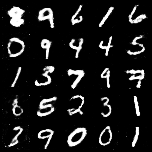
\includegraphics[width=\textwidth]{img/p2t2/187500.png}
    \caption{End ($187,500/187,500$)}
  \end{subfigure}
  \caption{Task 2 Training Process}
  \label{fig:p2t2_train}
\end{figure}

\subsection{Result Analysis}

\subsubsection{Overall Analysis}

It can be intuitively seen from the figure that: at the very beginning, the so-called "images" generated are just simple noise points, which have nothing to do with the MNIST handwriting data set

When the training reaches half (approximately $20,000 \sim 90,000$ iterations), the Generator has been able to generate images that are similar to the handwritten digits data set, but there is some noise and the shape of the handwritten digits is not very stable.

When the training is completely completed (approximately $180,000$ iterations), compared with the first two, there are fewer noise points, and the shape of the handwritten numbers is more specific and clear, indicating that the result of training is much better.

\subsubsection{Training Analysis}

Observing the output image, we can find that in the initial stage of training, the  influence of learning is relatively great. The noise that was still meaningless at about $10,000$ iterations, had begun to take on a digital shape by $20,000$ iterations.

But comparing $90,000$ and $180,000$, the marginal diminishing effect appears clearly: compared with the previous training, the gap between them is not very obvious, and even after training for $180000$ iterations, the generation of handwritten data still has not a completely clear part.

\subsubsection{Network Analysis}

One consideration is the structure of my GAN network itself. In fact, in this assignment , following the suggestions on the template, I used linear layers as the main part of the network. According to the comparison of Assignment 2, we already know that in problems related to image processing, convolutional layers often has better results than linear layers. So I think that if I use the convolutional generator structure such as Fig \ref{fig:p2_gan_struct}, I may get better image generation results.

\section{Part 2 Task 3}

\subsection{Simple Introduction}

In this part, I need to sample 2 images from my GAN. Interpolate between these two digits in latent space and include the results in my jupyter notebook. Use 7 interpolation steps, resulting in 9 images (including start and end point).

\subsection{Generate Strategy Analysis}

\subsubsection{Strategy Introduction}

In this part of the implementation, I first randomly generate two noises with length \texttt{latent\_dim} as the begin and end noise, then interpolate 7 noises averagely between the two noises, and finally generate the results through the Generator.

\subsubsection{Set notations}

\begin{itemize}
    \item $k$, \texttt{steps}, $9$ total steps to generate
    \item $n_1$, \texttt{noise\_begin}, begin noise
    \item $n_k$, \texttt{noise\_end}, end noise
\end{itemize}

\subsubsection{Define Expression}

\begin{align}
    \alpha_i &= \frac{i-1}{k} (1 \leq i \leq k) \\
    n_i &= (1 - \alpha_i) \cdot n_1 +\alpha_i \cdot n_k 
\end{align}

Then the generator use noise $n_1 \ldots n_k$ to generate $k$ images respectively.

\subsection{Result Visualization}

Figure \ref{fig:p2t3_results} shows some results.

\begin{figure}[!htbp]
  \centering
  \begin{subfigure}[b]{0.85\textwidth}
    
\includegraphics[width=\textwidth]{img/p2t3/whole1.png}
    \caption{Case 1 (7 to 8)}
  \end{subfigure}
  \begin{subfigure}[b]{0.85\textwidth}
    
\includegraphics[width=\textwidth]{img/p2t3/whole2.png}
    \caption{Case 2 (1 to 7)}
  \end{subfigure}
  \begin{subfigure}[b]{0.85\textwidth}
    
\includegraphics[width=\textwidth]{img/p2t3/whole3.png}
    \caption{Case 3 (0 to 5)}
  \end{subfigure}
  \caption{Task 3 Sample Results}
  \label{fig:p2t3_results}
\end{figure}

\subsection{Result Analysis}

\subsubsection{Generate Analysis}

We can see that if the first and last noises correspond to two different digital shapes, then the value in the middle will be generated as the shape between the two, showing a transition-like behavior.

In the process of generating images, the interpolation noise generated by my strategy may also be randomly generated directly. In this case, such a image looks like a number and another number. But the number image do not directly exist in the MNIST data set which is used for training. As a result, GAN is like generating a non-existent image  out of thin air.

\subsection{Application Analysis}

With this extension of Assignment, we can imagine that GAN can be applied to generate realistic world images, including human faces, animals, natural scenery, etc. It can even learn a certain artistic style or type of pictures to generate new pictures similar to this style. In this way, GAN can also be used as an implementation method for the recently popular AI painting.

But this "learning" is also controversial. MNIST in this assignment is an academic open source data set, and it is understandable to use it for GAN training. But for works of an artist with obvious style, or facial portraits, will the copyright or portrait rights of others be infringed during the learning process?

Although these problems are not directly related to the academic content of deep learning, it is also a point that has to make people think deeply.

\bibliographystyle{plain}
\bibliography{references}

\newpage

\begin{appendix}

\section{Extra Pictures}

\begin{figure}[!htbp]
  \centering
  \begin{subfigure}[b]{1\textwidth}
    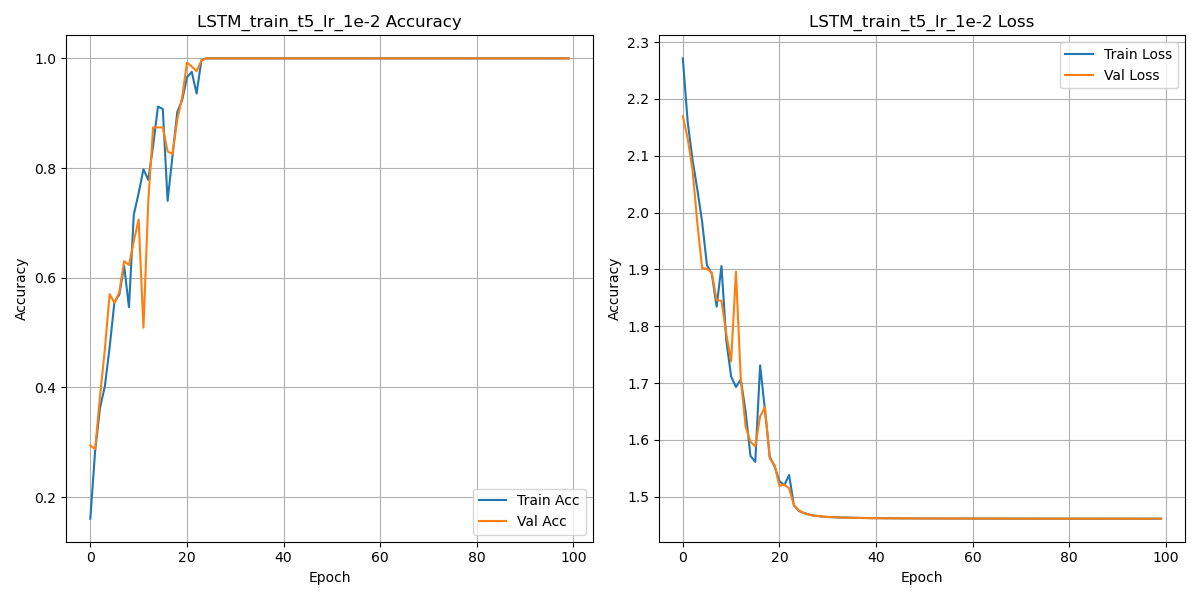
\includegraphics[width=\textwidth]{img/part1/LSTM_train_t5_lr_1e-2.png}
    \caption{Learning Rate $1\mathrm{e}^{-2}$}
  \end{subfigure}
  \begin{subfigure}[b]{1\textwidth}
    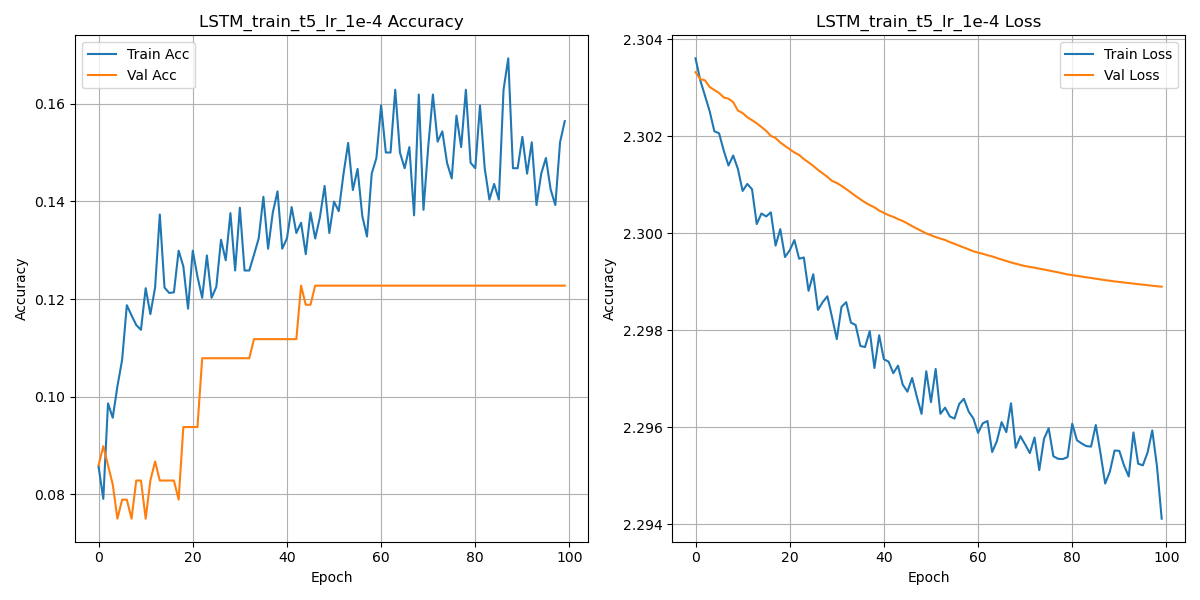
\includegraphics[width=\textwidth]{img/part1/LSTM_train_t5_lr_1e-4.png}
    \caption{Learning Rate $1\mathrm{e}^{-4}$}
  \end{subfigure}
  \caption{$T = 5$ Change Learning Rate Curve}
  \label{fig:p1_t5_lr_change}
\end{figure}

\begin{figure}[!htbp]
  \centering
  \begin{subfigure}[b]{1\textwidth}
    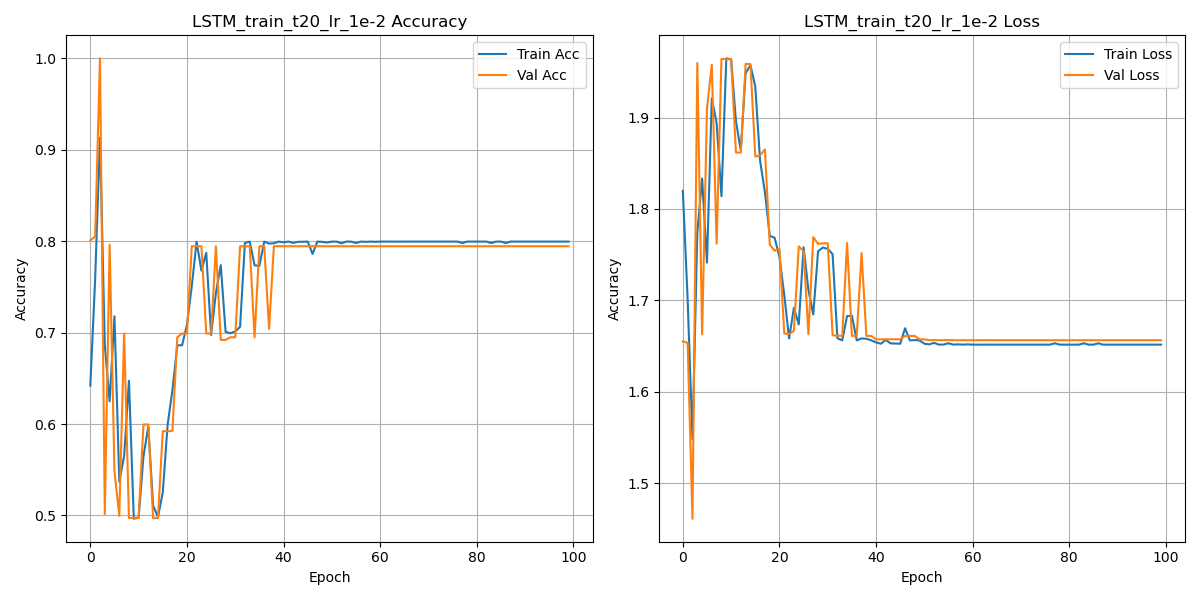
\includegraphics[width=\textwidth]{img/part1/LSTM_train_t20_lr_1e-2.png}
    \caption{Learning Rate $1\mathrm{e}^{-2}$}
  \end{subfigure}
  \begin{subfigure}[b]{1\textwidth}
    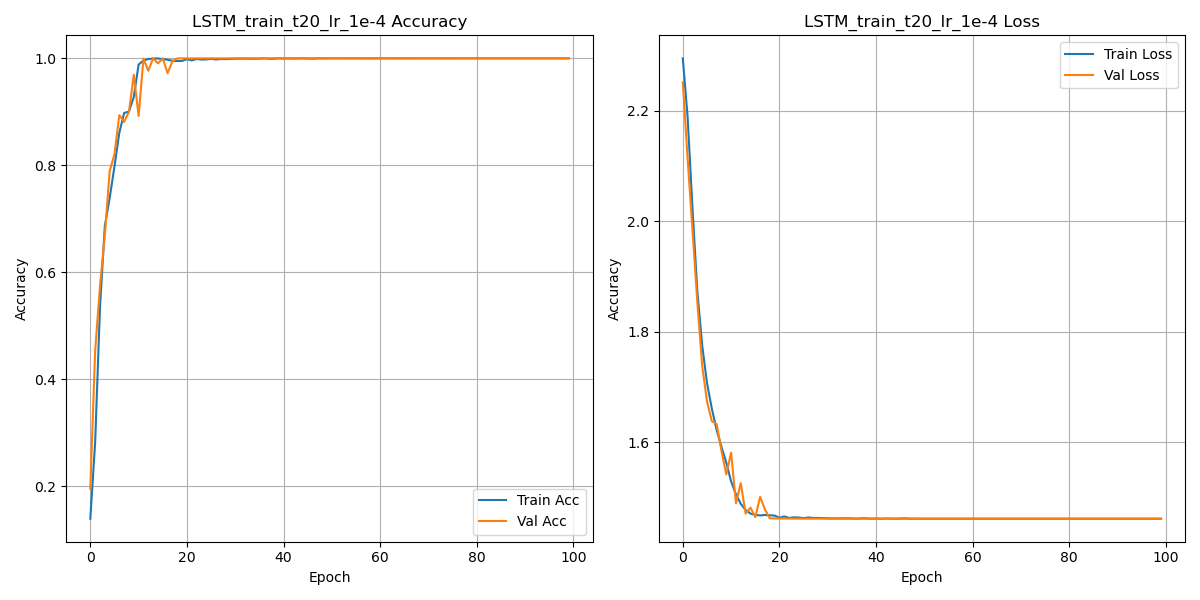
\includegraphics[width=\textwidth]{img/part1/LSTM_train_t20_lr_1e-4.png}
    \caption{Learning Rate $1\mathrm{e}^{-4}$}
  \end{subfigure}
  \caption{$T = 20$ Change Learning Rate Curve}
  \label{fig:p1_t20_lr_change}
\end{figure}

\begin{figure}[!htbp]
    \centering
    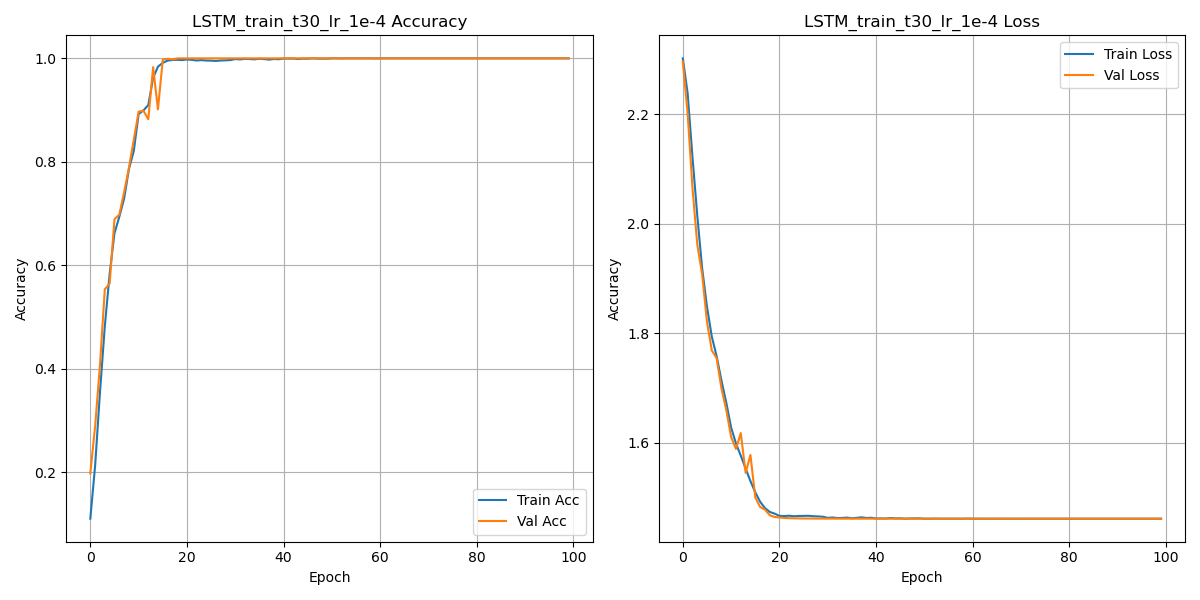
\includegraphics[width=1\textwidth]{img/part1/LSTM_train_t30_lr_1e-4.png}
    \caption{$T = 30$ Learning Rate $1\mathrm{e}^{-4}$ Curve}
    \label{fig:p1_t30}
\end{figure}

\begin{figure}[!htbp]
    \centering
    \includegraphics[width=1\textwidth]{img/part1/RNN_train_t20_default.png}
    \caption{$T = 20$ RNN Curve}
    \label{fig:p1_t20_rnn}
\end{figure}

\end{appendix}

\end{document}

